Building this application different architectural styles and patterns have been used.
\subsection{4-tier JEE client-server architecture}
	This architectural style has been used for separating efficiently the different levels of execution. The components of the application are identified in this tiers:
	\begin{itemize}
		\item{Client tier: is the layer that interact with the users. It runs on the client machine. This layer contains the On-Board computer, the Mobile application and the Web application.}
		\item{Web tier: is the layer that manage the interaction between the Web application and the Business tier. It contains Servlets, JSP pages and JavaServer Faces. In our system it is implemented by the Web server.}%giusto definire cosi' la cosa?
		\item{Business tier: contains Java Beans and Java Persistence Entities. It receives data from client programs, processes it (if necessary), and sends it to the enterprise information system tier for storage. An enterprise bean also retrieves data from storage, processes it (if necessary), and sends it back to the client program. In our system it is implemented by the Application server.}
		\item{Enterprise Information System tier: runs EIS software and includes enterprise infrastructure systems, such as enterprise resource planning (ERP), mainframe transaction processing, database systems, and other legacy information systems. It represents the data layer. The MySQL Database server is chosen for the creation and the maintainance of all the application data.}
	\end{itemize}
	\begin{figure}[!ht]
  \centering
  \vspace{0.2cm}
  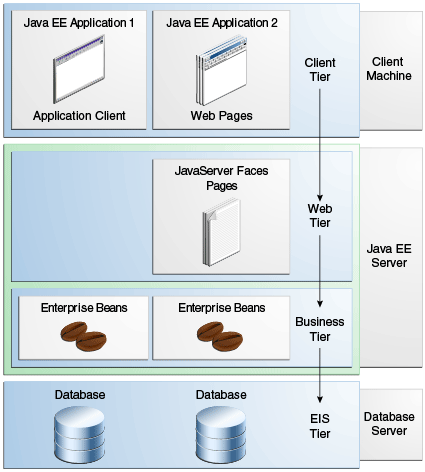
\includegraphics[width=0.6\textwidth]{/DD/jee_architecture}\\
  \vspace{0.4cm}
  \caption{Components Diagram} 
  \label{fig:Architecture of the system} 
\end{figure}
\subsection{Client-Server}
	The client-server communication model is highly used in this application.
	The On-Board computer and the Mobile application are clients with respect to the Application Server. The Web application consist of a Web browser that is a client with respect to the Web Server. The Web server is also a client with respect to the Application server. The Database is a server with respect to the Application server that act as a client.
\subsection{Thin client}
	In order to avoid that the client machine is involved in any logic decision we decided that all the computations will be run in the Application server. This comports different important advantages for the client tier: the client application will comport lower operational cost for the device, a superior security is obtained, the data are synchronized and the system is highly reliable. In addition this make the application independent from the number of clients connected.
\subsection{MVC}
	The Model-View-Controller pattern has been used in this application during the implementation of the client tier. In this way we separated the model, that rapresent the knowledge, the view, that is a visual representation of the model, and the controller, that is the link between a user and the system.
